\begin{figure}[H]
	\centering
	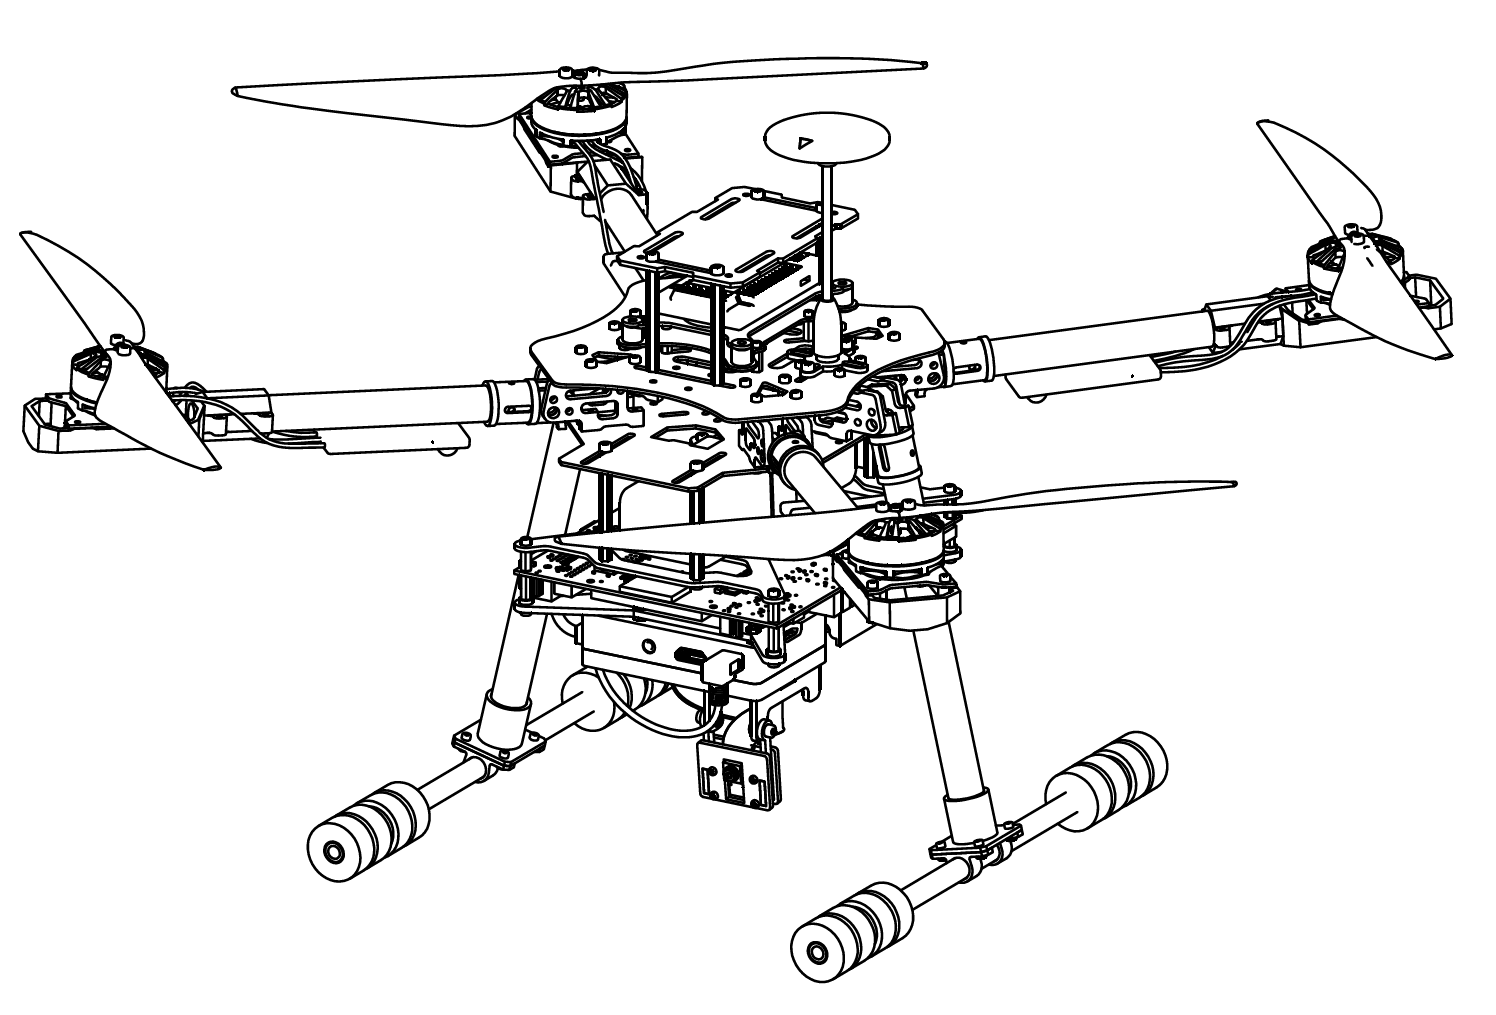
\includegraphics[width=0.85\textwidth]{img/multirotor.png}
	\caption[Team 109 Multirotor Drone]{Team 109 Multirotor Drone}
	\label{fig:drone1}
\end{figure}

A remote-piloted aerial system (RPAS) or sometimes referred to as ``drone" and ``multirotor" consists of serveral subsystems: the airframe, mechanical structures, propulsion, battery, sensors, and flight computer. This section will explore these subsystems in more detail. Figure~\ref{fig:drone1} is a render of the completed multirotor with the computing platform payload attached.

\subsubsection{Mechanical}\label{section:drone-mech}

The frame and mounts which holds the propulsion system, on-board computer/sensors, and the payload together makes up most of the mechanical subsystem of the multirotor.

\paragraph{Frame Configuration}

\begin{figure}[b]
	\centering
	\begin{subfigure}[b]{0.3\textwidth}
		\centering
		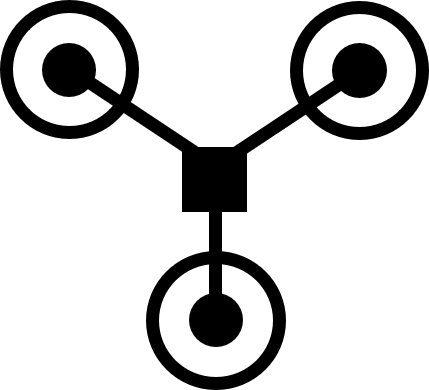
\includegraphics[scale=0.4]{img/drone_yconfig}
		\caption{Tricopter Y-Configuration}
		\label{fig:tricopter-y}
	\end{subfigure}
	~
	\begin{subfigure}[b]{0.3\textwidth}
		\centering
		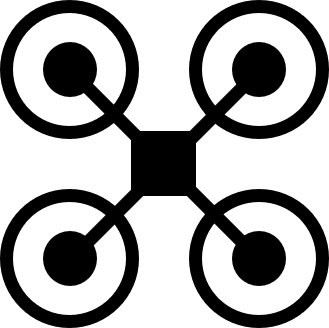
\includegraphics[scale=0.4]{img/drone_xconfig}
		\caption{Quadcopter X-Configuration}
		\label{fig:quadcopter-x}
	\end{subfigure}
	~
	\begin{subfigure}[b]{0.3\textwidth}
		\centering
		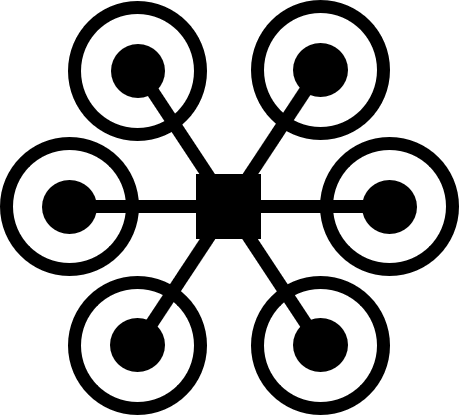
\includegraphics[scale=0.4]{img/drone_hexconfig}
		\caption{Hexcopter X-Configuration}
		\label{fig:hexcopter-x}
	\end{subfigure}
	
	\caption{Multirotor RPAS Configurations}
	\label{fig:rpas-config}
\end{figure}

\begin{figure}[h]
	\centering
	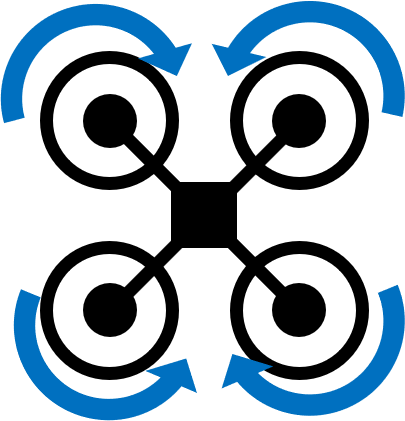
\includegraphics[scale=0.4]{img/drone_xconfigt}
	\caption{Quadcopter X-configuration}
	\label{fig:quadcopter-x-t}
\end{figure}

\begin{figure}[h]
	\centering
	\begin{subfigure}[b]{0.3\textwidth}
		\centering
		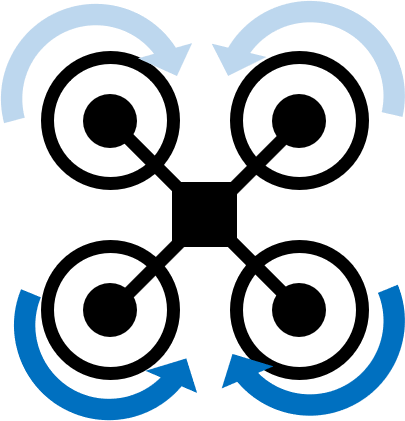
\includegraphics[scale=0.4]{img/drone_x_pitch}
		\caption{Pitch forward}
		\label{fig:x-pitch}
	\end{subfigure}
	~
	\begin{subfigure}[b]{0.3\textwidth}
		\centering
		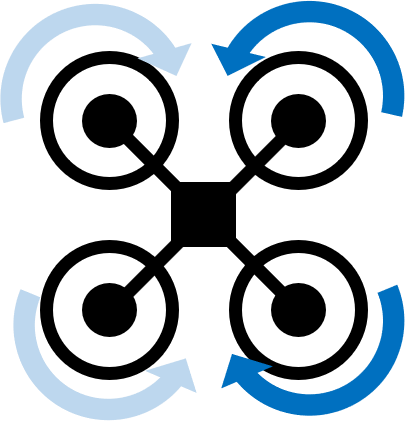
\includegraphics[scale=0.4]{img/drone_x_roll}
		\caption{Roll left}
		\label{fig:x-roll}
	\end{subfigure}
	~
	\begin{subfigure}[b]{0.3\textwidth}
		\centering
		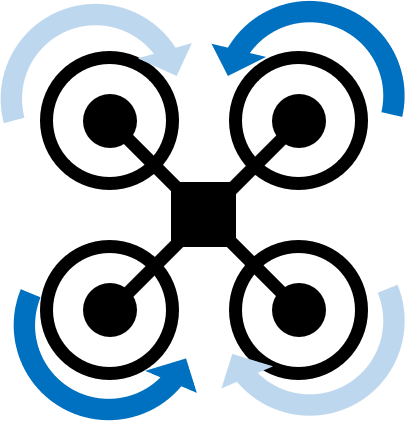
\includegraphics[scale=0.4]{img/drone_x_yaw}
		\caption{Yaw left}
		\label{fig:x-yaw}
	\end{subfigure}
	
	\caption{Using differential thrust to achive 6-DOF movement. }
	\label{fig:rpas_6dof}
\end{figure}

Multirotors have different configurations such as tricopter, quadcopter, hexacopter as depicted in Figure~\ref{fig:rpas-config}. As each frame has different motor layouts, the forces acting on the multirotor are inherently different and thus each configuration provides particular advantages and disadvantages.

We use a quadcopter X4 configuration (4 motors and propellers in the shape of a letter X) for our multirotor because it is easy to control and provides abundant control system robustness. Such configuration is also the most popular amongst the UAS industry because for its balance between redundancy and robustness with capacity and performance.

Figure \ref{fig:quadcopter-x-t} shows an example of the X4 configuration. Two of the motors spin clockwise and the other two spin counter-clockwise --- effectively canceling each other's unintended torque to the multirotor. Applying the same power into each motor allows the MRPAS to hover in place. We can perform 6 degree-of-freedom (DOF) movements by applying a combination of differential thrusts to each motor (Figure \ref{fig:rpas_6dof}). An X4 configuration is thus inherently stable.

A dual-blade helicopter, for example, requires the fewest number of motors. Like a single-blade helicopter, the system (in control theory sense) is naturally unstable and instills difficulty to stabilize the system. A tricopter has an odd number of motors --- sharing similar characteristics with a helicopter where the system requires an additional tail motor to compensate for the uneven torque. 

Configurations using more than 4 motors (such as hexacopters or octocopters) are very expensive for the amount of parts they require, however they fly more stablily and has failure redundancies. These drones are typically much larger (0.6m to 1.5m wide) and much heavier (up to 25 kg). As a result, they are typically used in industrial, filming, and agricultural applications with a typical unit cost of thousands of dollars. These configurations are not suitable for our applications.

\paragraph{Airframe}

\begin{figure}[h]
	\centering
	\begin{subfigure}[b]{0.33\textwidth}
		\centering
		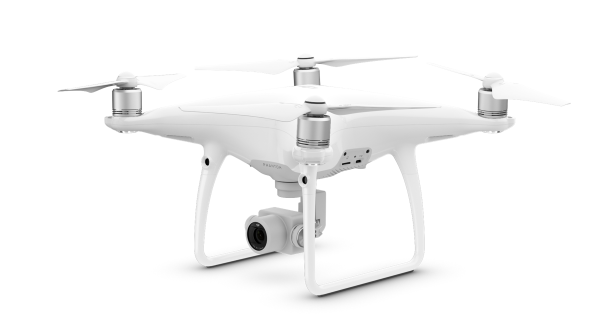
\includegraphics[width=\textwidth]{img/djiphantom4}
		\caption{DJI Phantom 4 (350 mm)}
		\label{fig:djiphantom}
	\end{subfigure}
	~
	\begin{subfigure}[b]{0.33\textwidth}
		\centering
		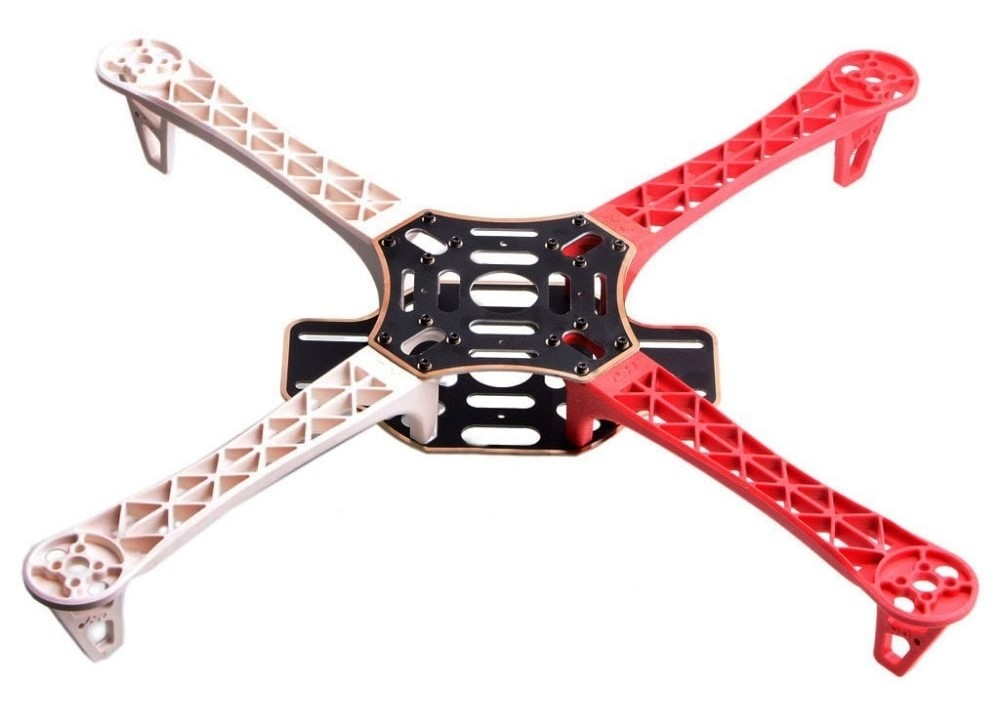
\includegraphics[width=\textwidth]{img/f450frame}
		\caption{Generic DIY frame kit (450 mm)}
	\end{subfigure}
	~
	\begin{subfigure}[b]{0.33\textwidth}
		\centering
		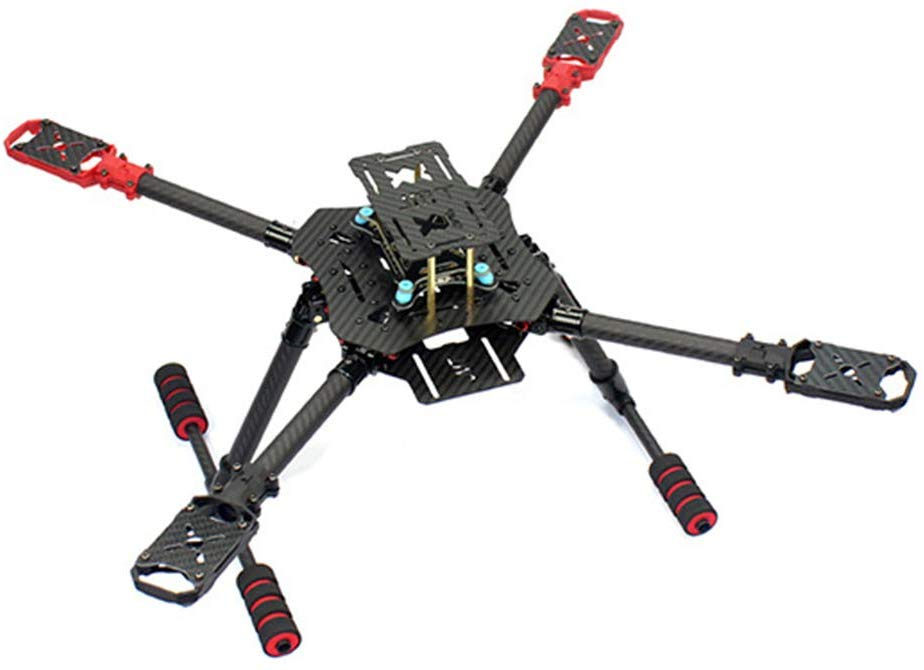
\includegraphics[width=\textwidth]{img/jmt560}
		\caption{JMT X4 Carbon Fiber Frame (560 mm)}
		\label{fig:jmtx4}
	\end{subfigure}
	~
	\begin{subfigure}[b]{0.33\textwidth}
		\centering
		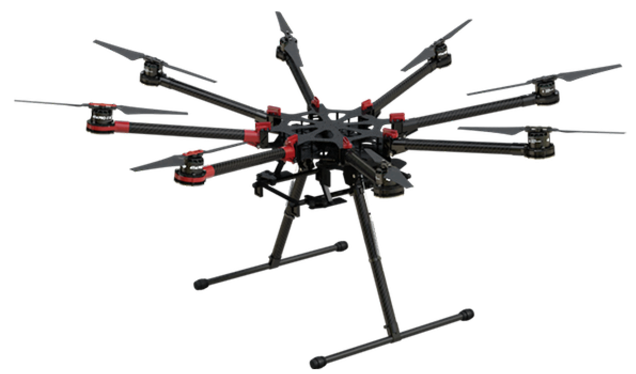
\includegraphics[width=\textwidth]{img/djis1000}
		\caption{DJI Spreadwings S1000 (1000 mm)}
		\label{fig:djis1000}
	\end{subfigure}
	
	\caption{Air Frame Options with and Their Sizes }
\end{figure}

Multirotor airframe sizes are commonly designated by their \textit{motor-to-motor-diagonal-span} (MMDS), which measures the distance between the pair of motors which are the furthest apart. 

We adopt a X4 560 mm MMDS carbon fibre frame from JMT, as shown in Figure~\ref{fig:jmtx4}. The frame is carbon fibre to enhance structural rigidity while keeping the system lightweight. The frame features foldable arms and landing gears for portability. Our client has the option to replace the brass hinges with static parts to reduce  weight and achieve a longer flight time. The X4 560 mm frame is also wide enough to support propellers up to 14 inches in diameter. The carbon fibre material is light, strong, and rigid. Although this means that the items mounted on the frame would suffer from lack of dampening of vibrations, we add compensating dampers for sensors separately.

The 350 mm frames are also popular amongst consumer products such as the DJI Phantom series\cite{dji-phantom-3-specs} as seen in Figure~\ref{fig:djiphantom}. A frame size of 350 mm would constrain our ability to mount larger hardware --- posing a significant risk to integrating computing platform hardware. The 350 mm size also limits the propeller size. The largest quadcopter configurations have an MMDS of 1000 mm to allow for extremely large payload capacities such as the one shown in Figure~\ref{fig:djis1000}; these are more commonly used for industrial or military applications.

\paragraph{Customized Add-ons}
% TODO: add CAD parts

\subsubsection{Propulsion}

The propulsion system covers the majority of the multirotor parts list and determines the flight performance of the multirotor. We refer to this subsystem as the ``Drive".

\paragraph{Motor Type}

Multirotors are electrically powered by a battery --- a DC source. Two common types of DC motors are  brushed motors and brushless DC (BLDC) motors. Brushed motors commutate mechanically using brushes whereas brushless motors commutate electrically using electronic controllers that switches phases in the stator coils. We use BLDC motors for their extended usable lifespan and efficiency. Brushed motors are not appropriate for our applications due to their excessive noise, friction, spark, and heat.

BLDC motors further consist of two variants: \textit{inrunner} and \textit{outrunner}. We choose outrunner BLDC motors for their higher torque output at lower speed  (i.e. outrunner motors have low KV constants; see Appendix~\ref{appendix:droneengine} for KV relationships). The lower speed of the rotor is beneficial for two reasons. One, a motor running at a lower speed is more efficient and produces fewer high frequency vibrations. Two, the attached propeller can be much larger and cut through the air at a lower speed, since drag forces acting on the blades are proportional to the velocity squared. While outrunner motors require more spin-up time as the rotor is more massive and has more inertia, this compromise is acceptable as the main operating mode of the multirotor is hovering, which requires little agility. 

The alternatives are inrunner motors, where the rotor is on the inside. Inrunner rotors are lighter and spin faster with a lower torque, thus requires gearboxes to extract useful torque\cite{invsoutrunner}.

\paragraph{Motor Size and Speed}\label{section:motor-speed}

Commercial outrunner BLDC motors generally have the following design parameters: stator size, KV/KT constants, voltage, maximum rated power, and weight. Please refer to Appendix~\ref{appendix:droneengine} for the relationship between the aforementioned design parameters. 

We choose 700 KV motors with stator size 3508.  According to drone hobbist online sources \cite{kv1, kv2}, the ideal KV motors to maximize performance for frame sizes larger than 450 mm should be 1200 KV or less. The argument of choosing a lower KV motor follows the point made above to balance torque output and energy loss due to air friction.

Our decision process consists of screening and ranking the best motors through applying priorities as follows:

\begin{enumerate}
    \item Voltage: We chose a motor that operates between 12.0 V and 20.0 V, which is sufficient for heavy operations.
    \item KV constant: Since the motors' RPM-per-volt ratio (KV constant) is inversely proportional of torque-per-current ratio (KT constant). We chose motors that have KV constants between 500 KV and 1000 KV. These constants are considered low-speed and high-torque, and are typically used for large drones and endurance flights. We also chose this range such that the propellers can spin slower and more efficiently, extending the maximum flight time.
    \item Rotor size: As mentioned in the previous section on inrunners vs. outrunners, larger rotors imply a lower KV and higher KT. As a result, we chose motors within the 500 KV to 1000 KV range. Markets show that sizes denoted 3508 to 2212 are adequate for this purpose.
    \item Maximum rated power: KV and KT constants are a simplified model for motor characteristics. The maximum power output is derived when considering realistic non-idealities such as heat, motor resistance, and mechanical limits. Typically 500 KV to 1000 KV motors have a rating between 150 W to 400 W, depending on the brand. We optimize for the most performant option allotted by our budget.
    \item Weight: Given that the weight of motors have little variance, we prioritize this parameter the least.
\end{enumerate}

\paragraph{Electronic Speed Controllers}

Electronic speed controllers (ESC) control the voltage, current, and phase supplied to a BLDC motor. As BLDC motors function by rotating magnetic fields using electric commutation, the ESCs must precisely control the timing and phase of the input. All ESCs function similarly and the design parameters are size/weight, power rating, power efficiency, and cost. We use HobbyWing X-Rotor 40.0 A ESCs. Figure \ref{fig:esc} from manufacturer's manual\cite{xrotoresc} shows an example of wiring. Note that instead of wiring to the recevier for direct control from the pilot, we connect the signal wires to the autopilot instead.

\begin{figure}[H]
	\centering
	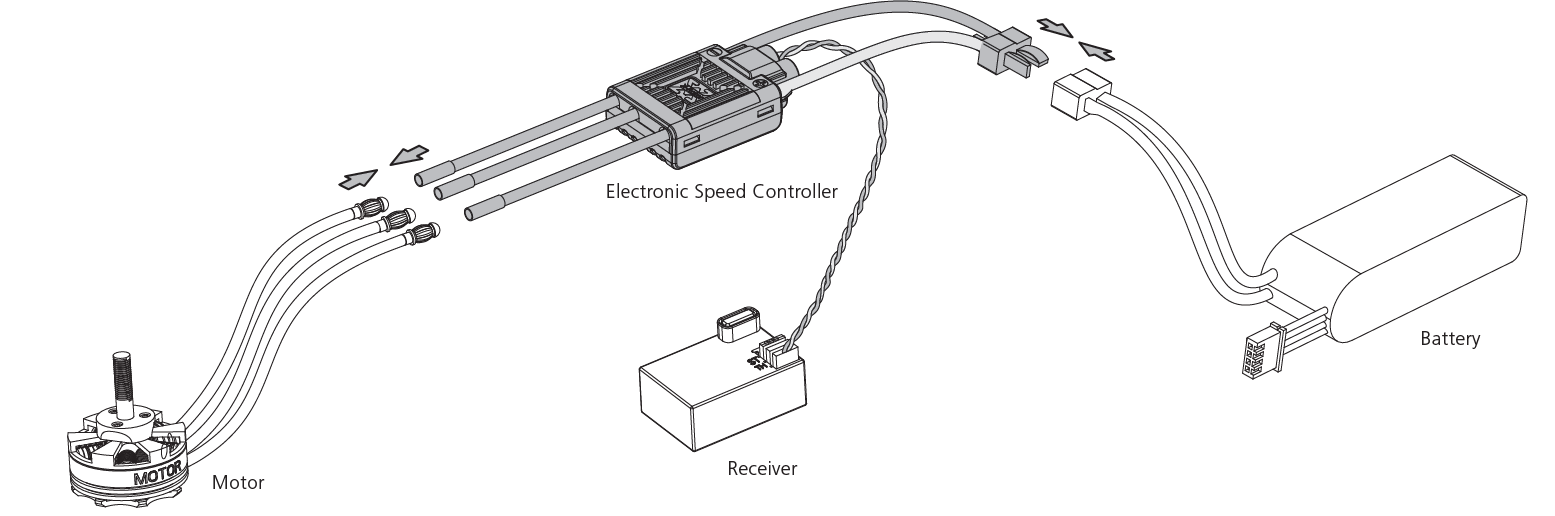
\includegraphics[width=\textwidth]{img/esc.png}
	\caption[Electronic speed controller]{Simplified Wiring of the Electronic Speed Controller, BLDC Motors, and the Battery}
	\label{fig:esc}
\end{figure}

\paragraph{Propellers}

Common RPAS propellers are made from plastic or carbon fibre. For the final deliverable we use carbon fiber propellers to maximize efficiency, flight time, and longevity for our client. 

Carbon fibre propellers are tough and rigid and produces efficient and low-noise flight performance\cite{cfvsp}.  While plastic propellers are cheap, abundant, and flexible, the manufacture of plastic propellers is not as precise, which leads to aerodynamic inefficiencies. Plastic propellers often require blade balancing, where one applies tape to the blades to balance the weight of each blade on the propeller. 

We choose propellers with size 1250, where 12 denotes 12 inches in diameter, and 50 denotes 5.0 inches in propeller pitch. To maximize thrust and minimize speed (seeing how low speed is more desirable, as mentioned in Section \ref{section:motor-speed}), we strike a balance if we choose 11 to 13 inch propellers to be fitted onto the multirotor.

\begin{figure}[h]
    \centering
    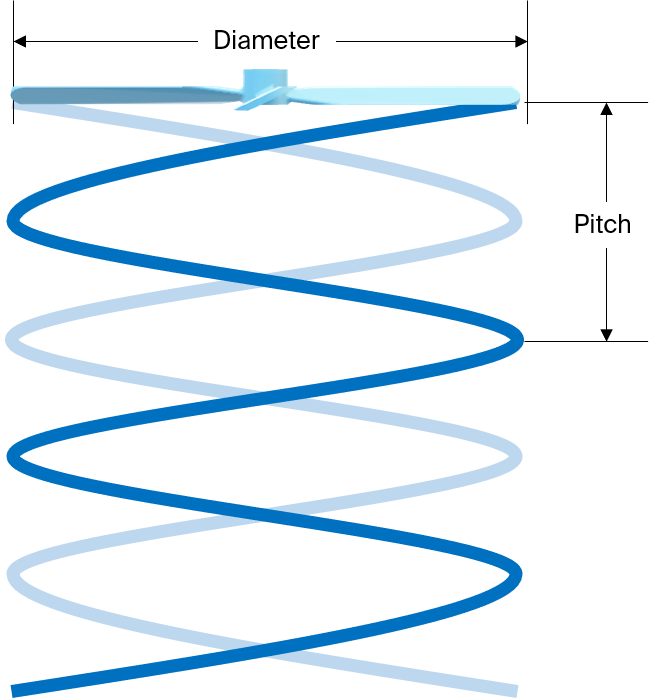
\includegraphics[scale=0.5]{img/proppitch}
    \caption{Propellor Diameter and Pitch Parameters}
    \label{fig:propeller}
\end{figure}

% TODO: update this graph
\begin{figure}[h]
    \centering
    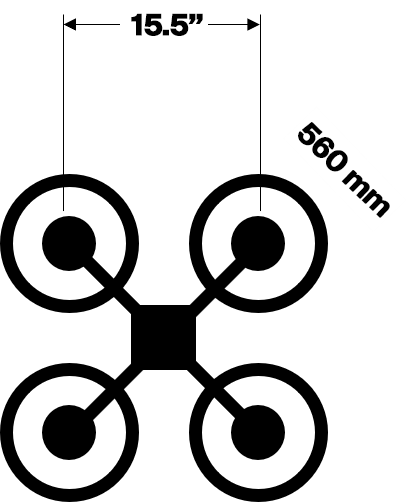
\includegraphics[scale=0.5]{img/framepropsize}
    \caption{Maximum Propeller Sizes}
    \label{fig:framepropsize}
\end{figure}

As mentioned in Section \ref{section:drone-mech} the frame size is 560 mm (22 inches), which means that the motor to motor adjacent span is about 15.5 inches (by dividing by $\sqrt{2}$). The  compatible size of propellers are between 11 to 14 inches to ensure several inches of clearance between propellers.

Mentioned in Section \ref{section:motor-speed}, we chose low-speed motors for their efficiency. Additionally recall that, given the same power, a slow-speed motor provides inversely proportional torque, so we chose propellers with high pitch (between 3 to 5 inches) to take advantage of the high-torque output in maximizing thrust output.

\subsubsection{Battery and Electrical Systems}

\paragraph{Battery}

\begin{figure}[h]
    \centering
    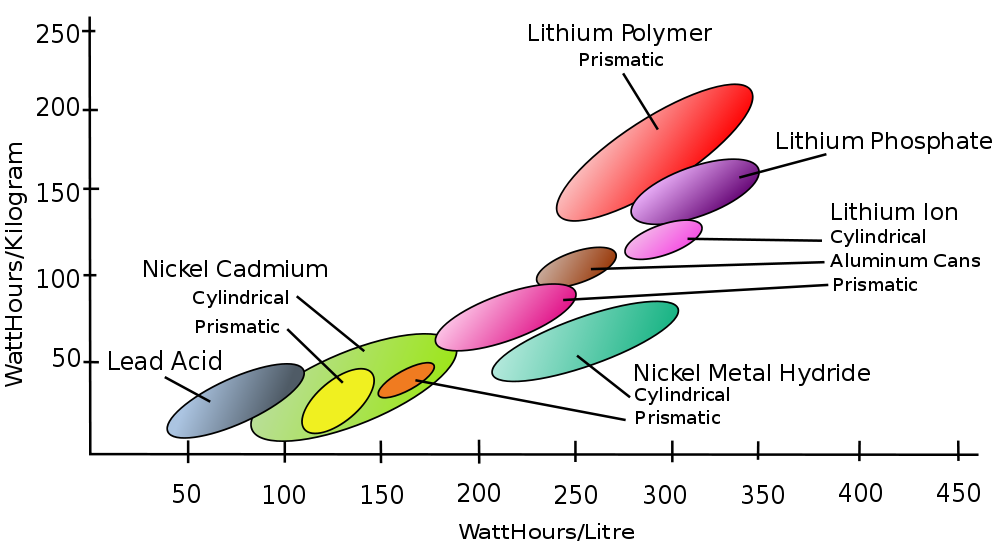
\includegraphics[width=0.5\textwidth]{img/energydensity.png}
    \caption{Energy Density Graph of Battery Types}
    \label{fig:batterytypes}
\end{figure}

We choose lithium polymer (Li-Po) batteries as they have the highest energy density (highest capacity to weight ratio), and are thus  perfect for high-power, low-weight applications. Figure~\ref{fig:batterytypes} shows a graph of the energy densities for differing types of batteries \cite{battery} --- from this graph, Li-Po batteries are the clear choice.


For a multirotor of this size, typical configurations include 3S and 4S (3 cells in series and 4 cells in series respectively) . As part of our deliverables (see List of Deliverables document), we provide a single 3S 5000 mAh battery with discharge rating of 30 C. The discharge rating indicates the maximum discharge current of the battery\cite{crate}:

$$
I_{max}=30 \times 5000 = 150~\text{A}
$$

\paragraph{Power Distribution}

Figure \ref{fig:pdb} depicts the layout of electrical power distribution for the multirotor subsystems. The 11.0 to 12.0 V from the 3S battery (or 14.0 to 15.0V of 4S batteries) is connected to a central PCB for power distribution. All the ESCs are to be connected in parallel to draw current from the battery. The power distribution board also has built-in voltage regulators for 5.0 V supply for digital flight hardware and other peripherals. The power distribution board is sandwiched between the flight controller unit/autopliot and the air frame as shown in Figure \ref{fig:pdb2}. Do not confuse the power distribution with the power supply for the payload. The power distribution shown here only supplies power to the multirotor subsystems and is independent of the PLB and PMB operations.

\begin{figure}[h]
    \centering
    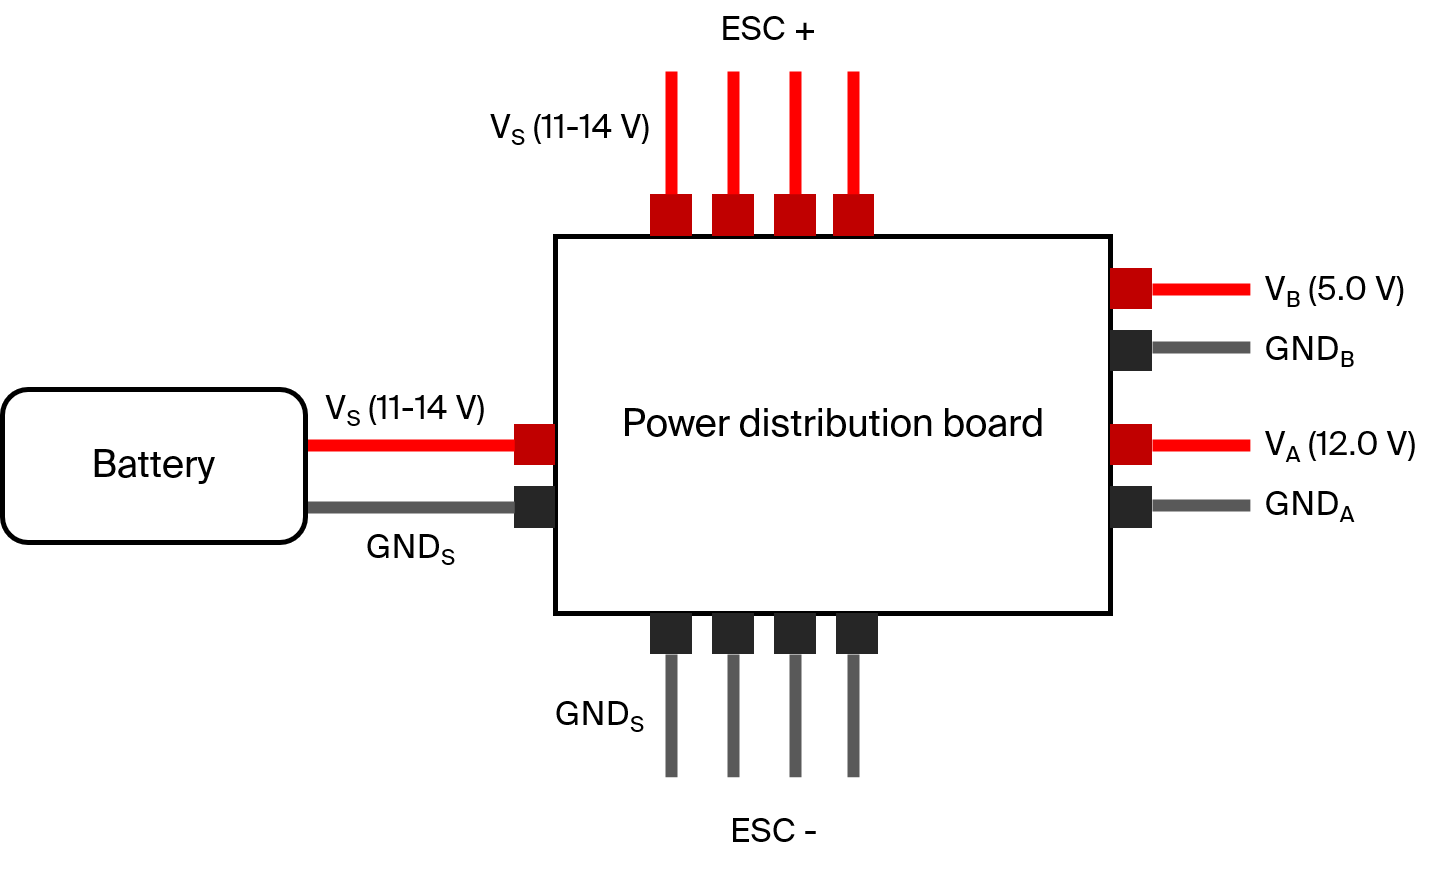
\includegraphics[width=0.6\textwidth]{img/pdb}
    \caption{Multirotor Power Distribution Layout}
    \label{fig:pdb}
\end{figure}

\begin{figure}[h]
    \centering
    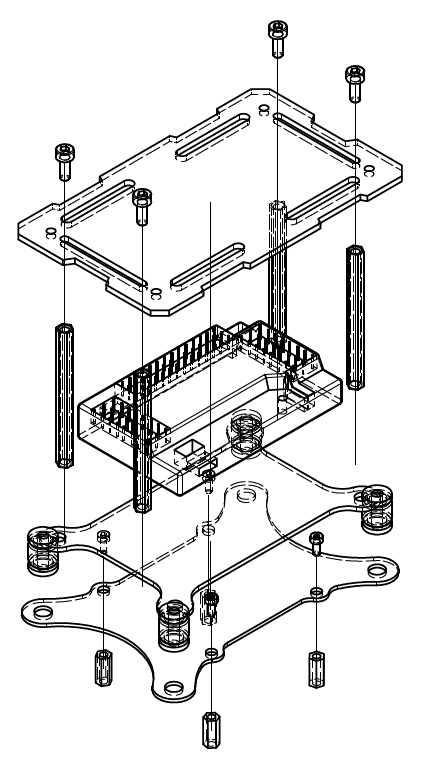
\includegraphics[width=0.4\textwidth]{img/pdb2}
    \caption{Multirotor Power Distribution Assembly Diagram}
    \label{fig:pdb2}
\end{figure}

\subsubsection{Flight Computer and Sensors}
% TODO: insert Ardell's text
\paragraph{Flight Computer Unit}
\paragraph{Sensors}
\paragraph{Flight Modes}
\paragraph{FCU Software}

\subsubsection{Communication and Control}

This subsection discuss the communication system on-board the multirotor used for multirotor control. Do not confuse this this communication link with base-station communication using the PMB and the base station web-app.
The multirotor communication link is independent from other systems to ensure modularity and compatibility in case of future upgrades.
The link uses 2.4 GHz radio with two end points: a receiver (RX) and transmitter (TX).

The transmitter is a RadioLink AT10 10-channel 2.4 GHz radio transmitter with colored display\cite{at10}. The multirotor receiver is a RadioLink R9DS 9-channel receiver\cite{r9ds}. Note that we use 6 out of 9 channel for normal operations.
The first four channels corresponds with each 4 axis of the flight controls: throttle, pitch, yaw, and roll. The last two channels, by default, corresponds with flight mode and return-to-home function respectively. 
The user has the option to add additional channels or remap the existing channels, see operations specifications (TODO: ref document) for steps on configuring the flight mode and radio channels using the autopilot software.

